\subsection{Enwicklung der Gui}
\FloatBarrier
Ein kurzer "Uberblick "uber die verschiedenen Stadien der Gui-Entwicklung.

\bigbreak
\bigbreak
\bigbreak
\bigbreak

\begin{figure}[h!]
	\centering
	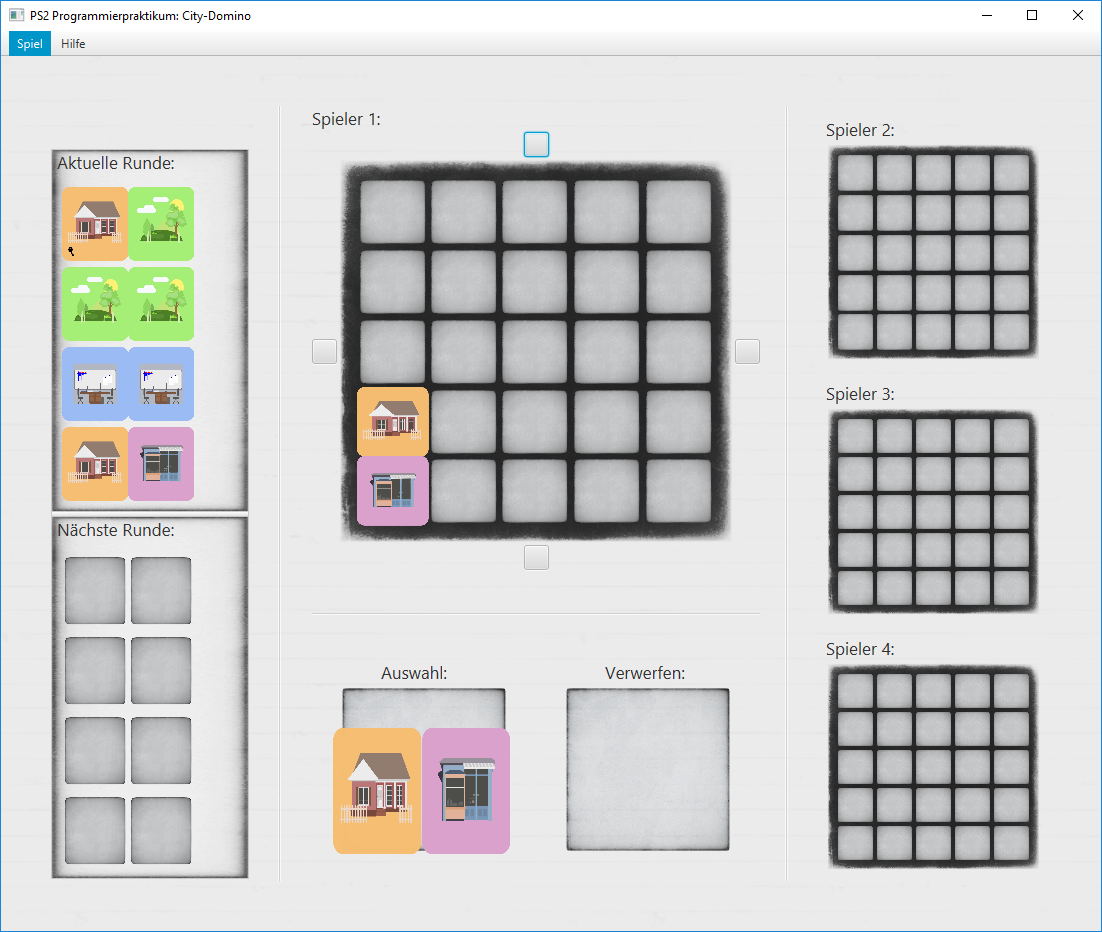
\includegraphics{anhang/pics/180918}
	\caption{Gui-Entwicklung 1}
	\label{fig:guiEnwicklung1}
\end{figure}

\begin{figure}
	\centering
	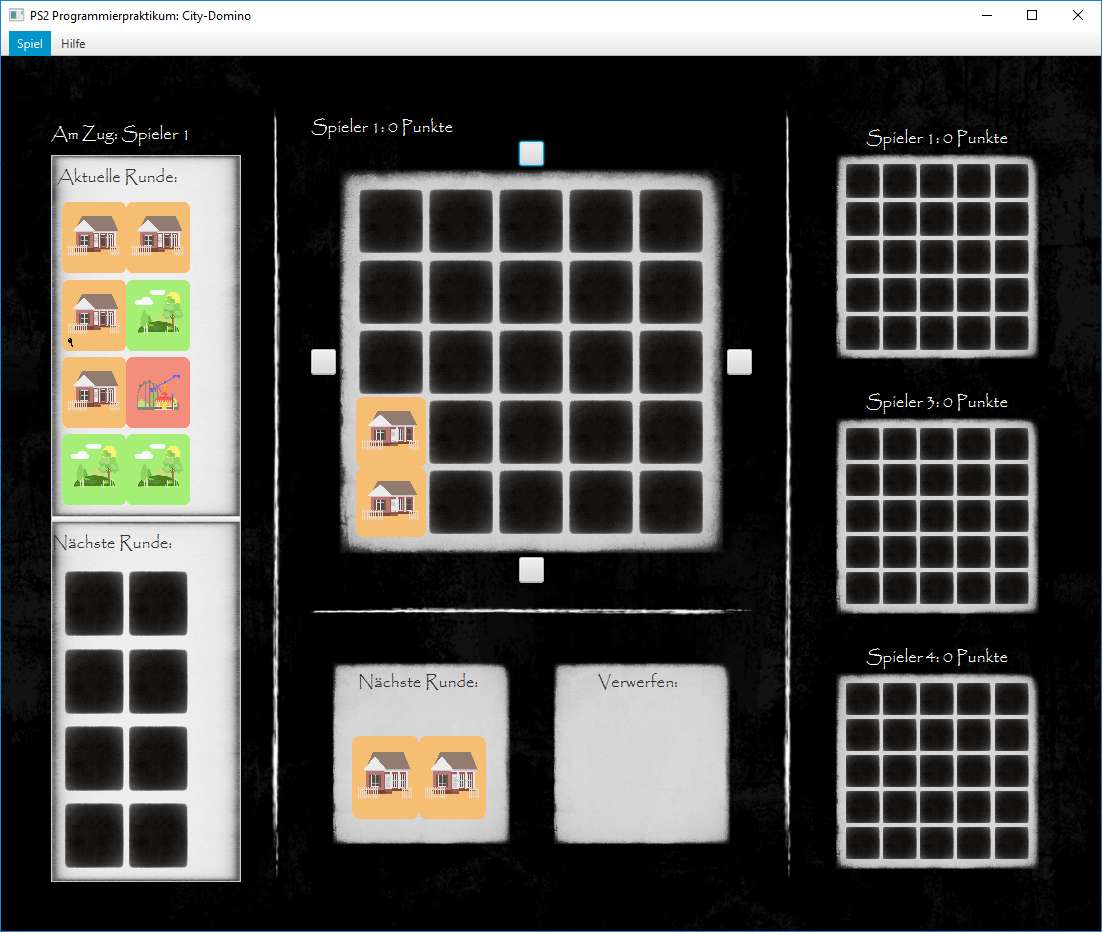
\includegraphics[width=0.75\linewidth]{anhang/pics/200918}
	\caption{Gui-Entwicklung 2}
	\label{fig:guiEnwicklung2}
\end{figure}

\begin{figure}
	\centering
	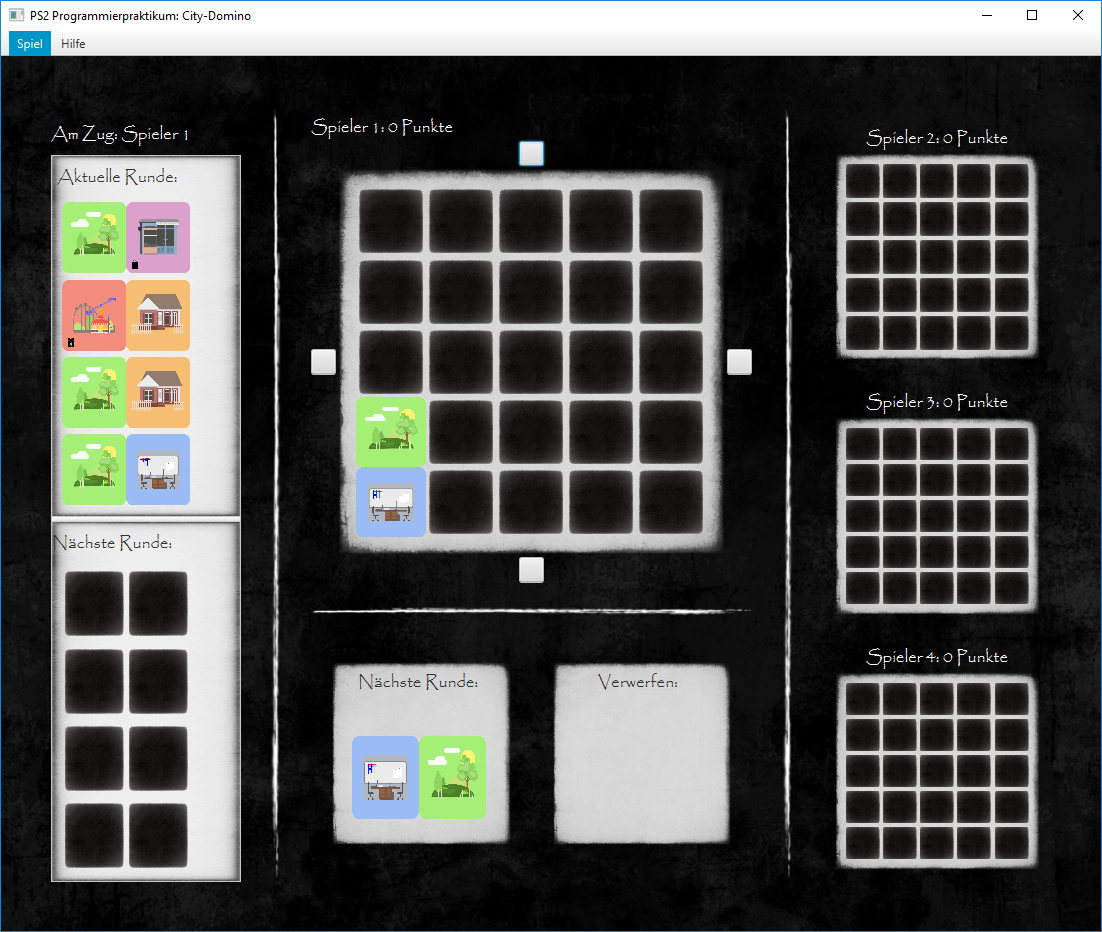
\includegraphics[width=0.75\linewidth]{anhang/pics/220918}
	\caption{Gui-Entwicklung 3}
	\label{fig:guiEnwicklung3}
\end{figure}

\begin{figure}
	\centering
	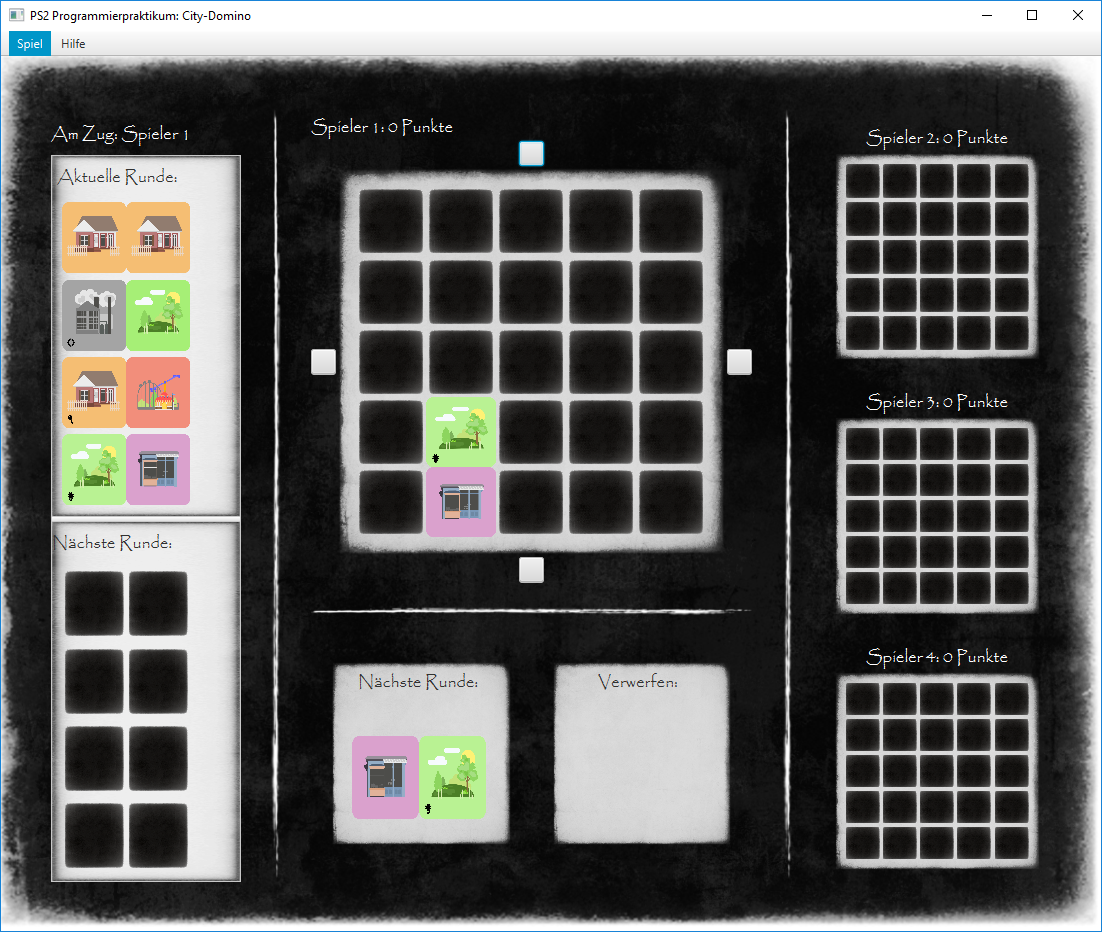
\includegraphics[width=0.75\linewidth]{anhang/pics/220918V2}
	\caption{Gui-Entwicklung 4}
	\label{fig:guiEnwicklung4}
\end{figure}

\begin{figure}
	\centering
	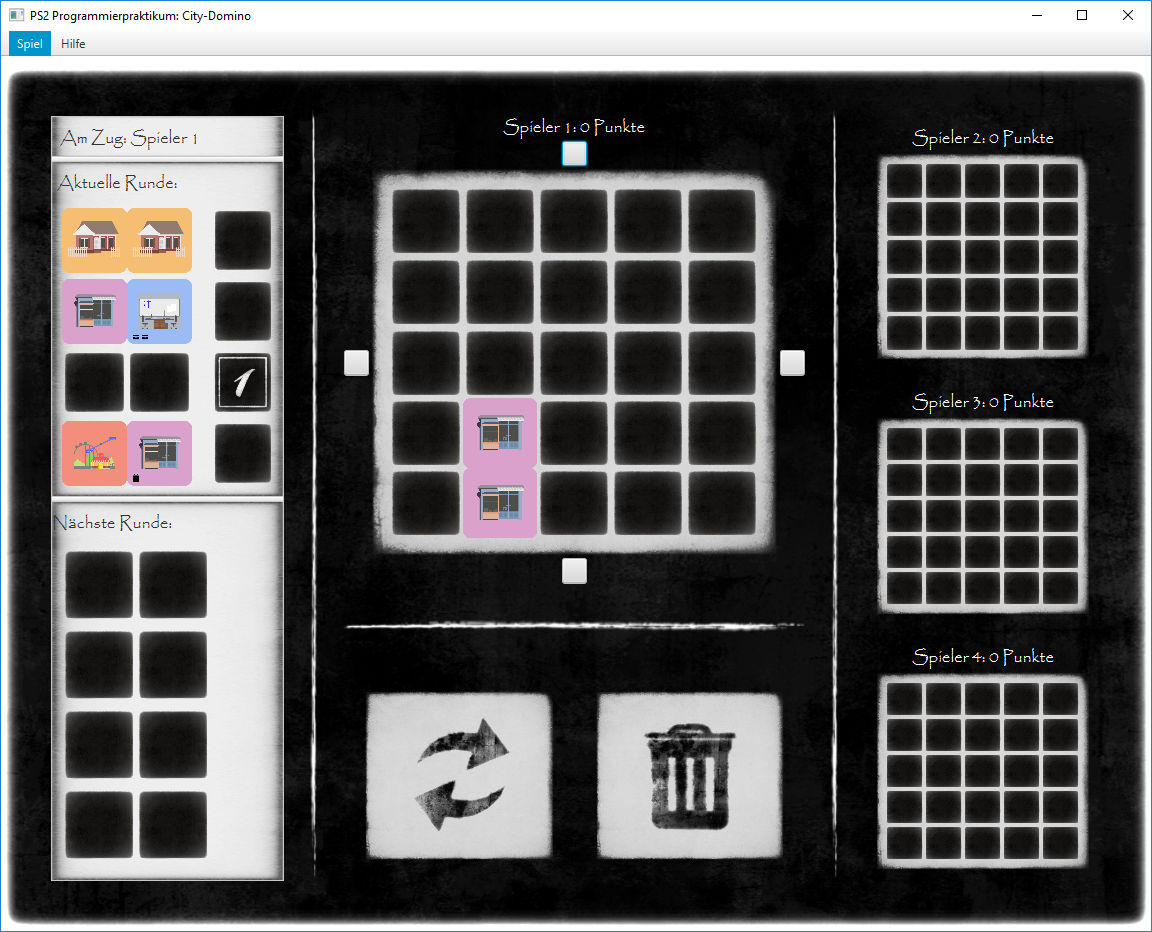
\includegraphics{anhang/pics/290918}
	\caption{Gui-Entwicklung 5}
	\label{fig:guiEnwicklung5}
\end{figure}

\begin{figure}
	\centering
	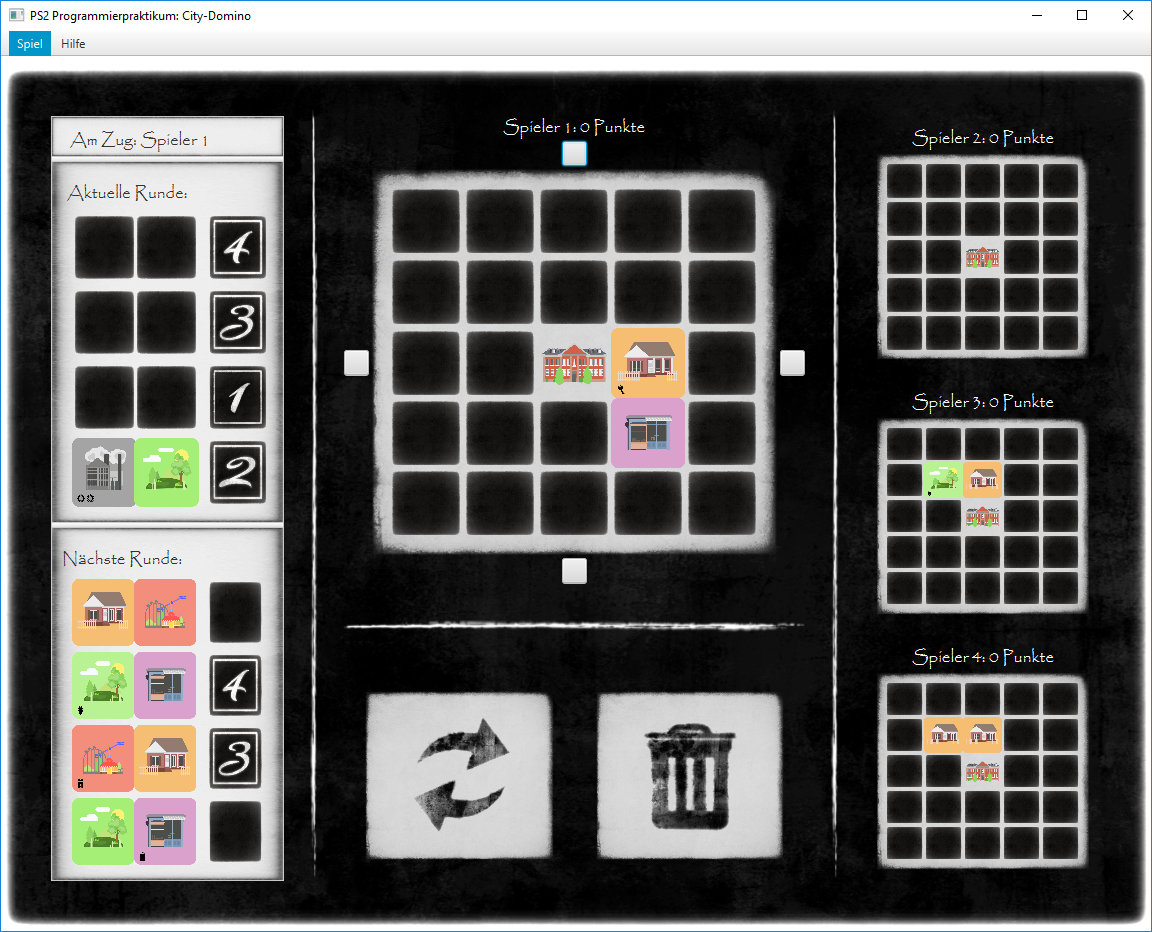
\includegraphics{anhang/pics/Main121018}
	\caption{Gui-Entwicklung 6}
	\label{fig:guiEnwicklung6}
\end{figure}

\begin{figure}
	\centering
	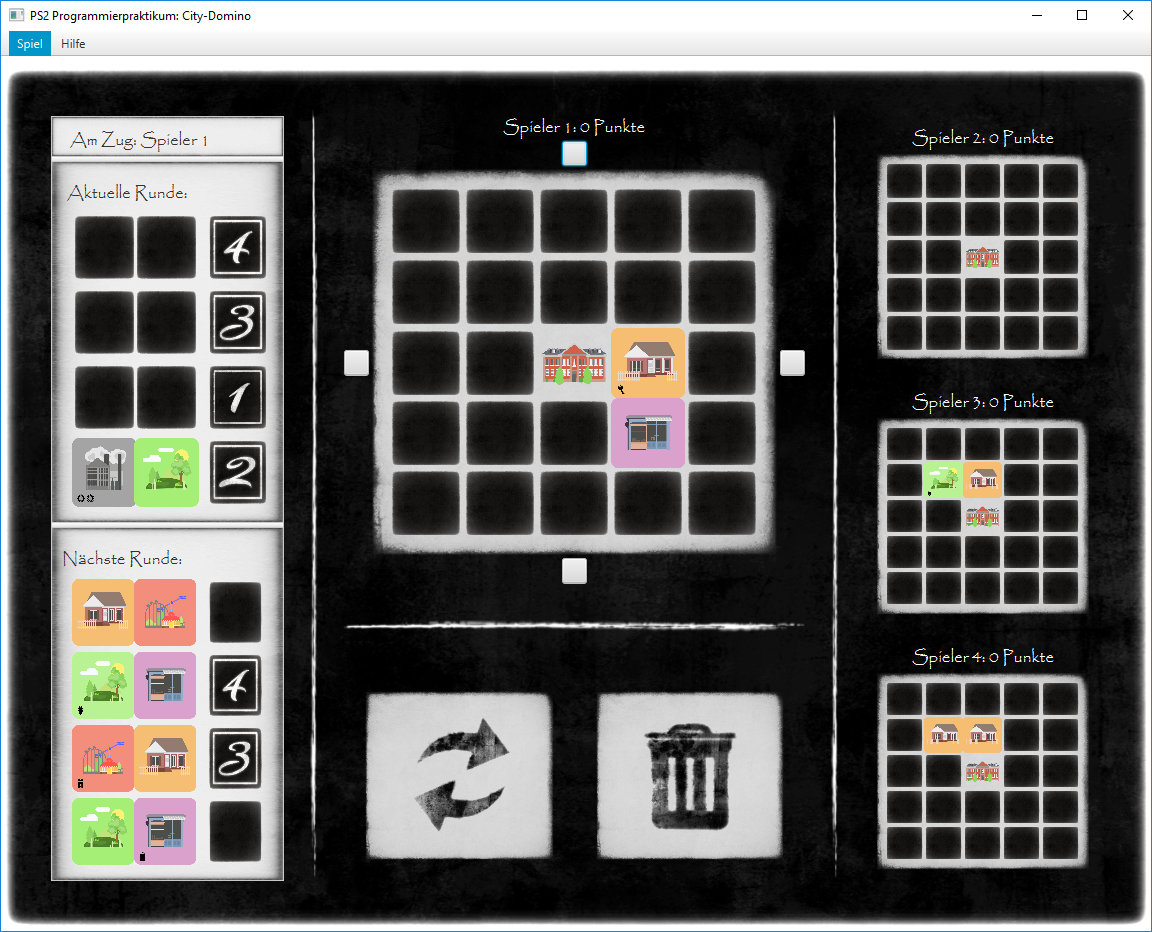
\includegraphics{anhang/pics/Main121018}
	\caption{Gui-Entwicklung 7}
	\label{fig:guiEnwicklung7}
\end{figure}

\begin{figure}
	\centering
	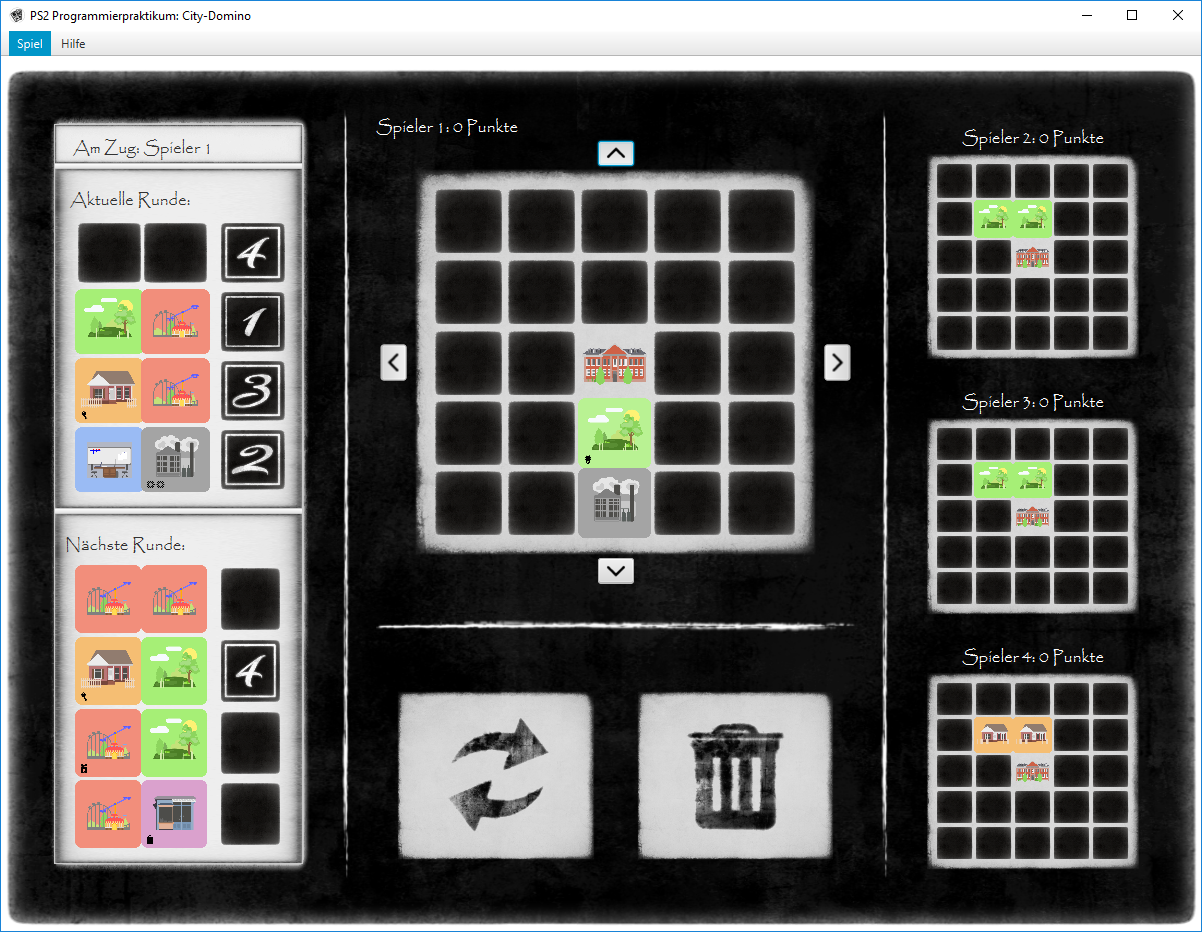
\includegraphics{anhang/pics/Main141018}
	\caption{Gui-Entwicklung 8}
	\label{fig:guiEnwicklung8}
\end{figure}